\pagestyle{empty}

% Header trang
\noindent
\textbf{\large 142} \qquad {\small\textsf{\textbf{CHƯƠNG 2}}} \quad {\small Giới hạn và Đạo hàm}
\vspace{16pt}\par

% Thiết lập 2 cột bất đối xứng: Cột trái 48mm (chứa hình), cột phải 134mm (chứa nội dung)
\setcolumnwidth{48mm, 134mm}
\setlength{\columnsep}{7mm}

\begin{paracol}{2}
% ==================== KHỐI 1 ====================
% Cột trái: Hình 3
\noindent
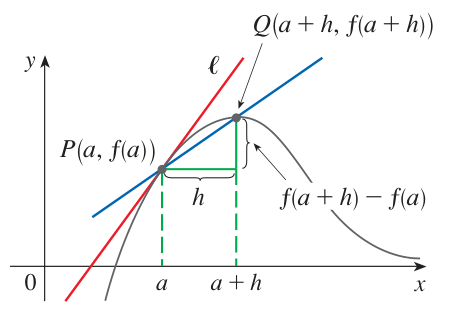
\includegraphics[width=\linewidth]{images/p0177_fig1.png}

\switchcolumn
% Cột phải: Dẫn nhập Công thức 2
\noindent
Có một biểu thức khác cho hệ số góc của tiếp tuyến mà đôi khi dễ sử dụng hơn. Nếu $h = x - a$, thì $x = a + h$ và do đó hệ số góc của cát tuyến $PQ$ là
\[
m_{PQ} = \frac{f(a + h) - f(a)}{h}
\]
(Xem Hình 3, trong đó trường hợp $h > 0$ được minh họa và $Q$ nằm ở bên phải của $P$. Tuy nhiên, nếu $h < 0$, thì $Q$ sẽ nằm ở bên trái của $P$.)

\vspace{1ex}
\noindent
Lưu ý rằng khi $x$ tiến tới $a$, thì $h$ tiến tới $0$ (vì $h = x - a$) và do đó biểu thức tính hệ số góc của tiếp tuyến trong Định nghĩa~1 trở thành

\vspace{1.2ex}
\begin{center}
\begin{tikzpicture}
  \node[draw=stewartred, line width=0.8pt, inner sep=7pt, minimum width=4.8cm] (eqbox) {
    $\displaystyle m = \lim_{h \to 0} \frac{f(a + h) - f(a)}{h}$
  };
  \node[draw=stewartred, line width=0.8pt, inner sep=2.5pt, rounded corners=0.5pt, left=1.8cm of eqbox.west] {
    \bfseries\textcolor{stewartred}{2}
  };
\end{tikzpicture}
\end{center}

\switchcolumn*
% ==================== KHỐI 2 ====================
% Cột trái: Hình 4 (dóng thẳng hàng với phần tính toán của Ví dụ 2)
\vspace*{3.6cm}
\noindent
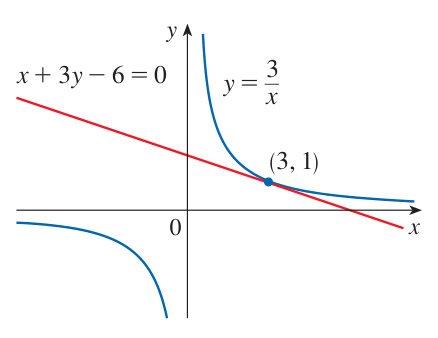
\includegraphics[width=\linewidth]{images/p0177_fig2.png}

\switchcolumn
% Cột phải: Ví dụ 2
\vspace{1ex}
\noindent
{\textsf{\textbf{\color{stewartblue}VÍ DỤ 2}}}\hspace{0.8em}Tìm phương trình tiếp tuyến của hyperbol $y = 3/x$ tại điểm $(3, 1)$.\par
\vspace{0.8ex}
\noindent
{\textsf{\textbf{\color{stewartblue}LỜI GIẢI}}}\hspace{0.8em}Đặt $f(x) = 3/x$. Khi đó, theo Công thức 2, hệ số góc của tiếp tuyến tại $(3, 1)$ là
\begin{align*}
m &= \lim_{h \to 0} \frac{f(3 + h) - f(3)}{h} \\[1ex]
  &= \lim_{h \to 0} \frac{\dfrac{3}{3 + h} - 1}{h} = \lim_{h \to 0} \frac{\dfrac{3 - (3 + h)}{3 + h}}{h} \\[1.5ex]
  &= \lim_{h \to 0} \frac{-h}{h(3 + h)} = \lim_{h \to 0} -\frac{1}{3 + h} = -\frac{1}{3}
\end{align*}

\noindent
Do đó, phương trình tiếp tuyến tại điểm $(3, 1)$ là
\[
y - 1 = -\frac{1}{3}(x - 3)
\]
\noindent
\rlap{rút gọn thành}\hfill $x + 3y - 6 = 0$\hfill\mbox{}

\vspace{1ex}
\noindent
Đường hyperbol và tiếp tuyến của nó được thể hiện trong Hình~4.\hfill{\color{stewartblue}\rule{1.2ex}{1.2ex}}

\switchcolumn*
% ==================== KHỐI 3 ====================
% Cột trái: Hình 5
\vspace{1ex}
\noindent
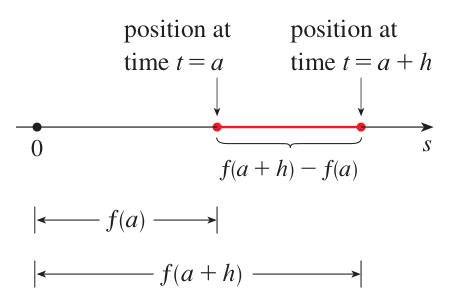
\includegraphics[width=\linewidth]{images/p0177_fig3.png}

\switchcolumn
% Cột phải: Mục Vận tốc
\vspace{1ex}
\noindent
{\color{stewartblue}\rule{1.1ex}{1.1ex}}\hspace{0.5em}{\large\textsf{\textbf{Vận tốc}}}\par
\vspace{0.8ex}
\noindent
Trong Mục 2.1, chúng ta đã khảo sát chuyển động của một quả bóng rơi từ tháp CN và định nghĩa vận tốc của nó là giá trị giới hạn của các vận tốc trung bình trên các khoảng thời gian ngày càng ngắn hơn.\par
\vspace{0.8ex}
\setlength{\parindent}{1.2em}
Nói chung, giả sử một vật chuyển động dọc theo một đường thẳng theo phương trình chuyển động $s = f(t)$, trong đó $s$ là độ dịch chuyển (khoảng cách có hướng) của vật tính từ gốc tọa độ tại thời điểm $t$. Hàm số $f$ mô tả chuyển động được gọi là \textbf{hàm vị trí} của vật. Trong khoảng thời gian từ $t = a$ đến $t = a + h$, sự thay đổi vị trí là $f(a + h) - f(a)$. (Xem Hình~5.)
\setlength{\parindent}{0pt}

\end{paracol}

\vfill
\begin{center}
{\fontsize{6.5pt}{8pt}\selectfont\color{darkgray}
Copyright 2021 Cengage Learning. All Rights Reserved. May not be copied, scanned, or duplicated, in whole or in part. WCN 02-200-203
}
\end{center}
